%% Section 2 of QM.tex (Quantum Mechanics Review). Compile QM.tex, not this file.
%% ============================================================
\section{Quantum Mechanics as an Example}
%% ============================================================

\paragraph{The quantum state is a vector in a Hilbert space.} A quantum state $|\Phi\rangle$ of a system with Hamiltonian $\hat H$ is an abstract \textcolor{blue}{state vector} in a Hilbert space $\mathcal{H}$, so the state obeys every rule in Table~\ref{tab:axioms}. The closure under addition is the superposition principle. The state itself is not measured. Measurements give values of the \textcolor{blue}{observables}, such as momentum, energy and angular momentum, and the state determines the probability of each value. Physics fixes the inner product of $\mathcal{H}$, because the probability $|\langle \Psi | \Phi \rangle|^2$ is measured. A formula that gave a different number in a different basis would, therefore, predict a different experimental result. Quantum mechanics calibrates the ruler with the position basis, $\langle \Psi | \Phi \rangle = \int dx\, \Psi^{*}(x)\, \Phi(x)$. The Born rule makes $|\Phi(x)|^2$ a probability density, so the squared length must be $\int dx\, |\Phi(x)|^2$. A Hermitian Hamiltonian also conserves the total probability, because the time evolution that the Hamiltonian generates is unitary under this inner product.

\paragraph{The wavefunction is the state written in the position basis.} The familiar wavefunction $\Phi(x)$ is not the state itself. The wavefunction is the \textcolor{blue}{position representation} of the state vector, and the other observables, such as momentum, can be calculated from it. Each value $\Phi(x)$ is the component of $|\Phi\rangle$ along the \textcolor{blue}{position eigenstate} $|x\rangle$:
\begin{equation}
    \boxed{\Phi(x) = \langle x | \Phi \rangle}
\end{equation}
The wavefunction is, therefore, a \textcolor{blue}{probability amplitude}. The value $\Phi(x)$ is a complex number, and the squared modulus $|\Phi(x)|^2$ is the probability density. The amplitude is the square root of the probability density, up to a phase $\theta(x)$:
\begin{equation*}
    \Phi(x) = \sqrt{|\Phi(x)|^2}\; e^{i\theta(x)}
\end{equation*}

\paragraph{The position eigenbasis is a continuous orthonormal basis.} The wavefunction is an infinite array with one complex number for each position $x$, with the position $x$ in the role of the index $i$ in Section~1. The sum over $i$ becomes an integral, and the Kronecker delta becomes the Dirac delta, $\langle x | x' \rangle = \delta(x - x')$. The completeness relation of the position eigenbasis is
\begin{equation*}
    \int dx'\, |x'\rangle\langle x'| = \mathbb{I}
\end{equation*}
Inserting the completeness relation in front of $|\Phi\rangle$ gives
\begin{equation*}
    |\Phi\rangle = \int dx'\, |x'\rangle\langle x' | \Phi \rangle
\end{equation*}
\begin{equation}
    \boxed{|\Phi\rangle = \int dx'\, \Phi(x')\, |x'\rangle}
\end{equation}
The primed variable $x'$ is a placeholder that runs over every position eigenstate, like the summation index $i$, and renaming $x'$ does not change the expansion. The unprimed variable $x$ is the single position at which the wavefunction is evaluated, like the fixed index $j$. The projection of the expansion back onto $\langle x|$, therefore, recovers one entry of the array:
\begin{align*}
    \langle x | \Phi \rangle &= \int dx'\, \Phi(x')\, \langle x | x' \rangle \\
    &= \int dx'\, \Phi(x')\, \delta(x - x') \\
    &= \Phi(x)
\end{align*}
The delta function selects the entry at $x' = x$ in the same way that the Kronecker delta $\delta_{ji}$ selects the component $v_j$. The position eigenstates are not normalizable, because $\langle x | x \rangle = \delta(0)$ diverges. Strictly, $|x\rangle$ lies outside $\mathcal{H}$, and the rigorous framework is the \textcolor{blue}{rigged Hilbert space}. The position eigenstates are still used as a basis, because every physical state is a normalizable superposition of them.

\paragraph{Discretizing the wavefunction turns the integral into a sum over array entries.} The array picture becomes concrete when the position axis is cut into points $x_i = i\,\Delta x$ with a small spacing $\Delta x$. Figure~\ref{fig:array} uses the wavefunction $\Phi(x) = \sqrt{2/\pi}\,\sin x$ on the interval $0 \leq x \leq \pi$, which is the ground state of an infinite square well of width $\pi$. Each point $x_i$ stores one number $\Phi(x_i)$, and the list of these numbers is a column vector with $N$ entries. The integral over $x'$ in the expansion of $|\Phi\rangle$ is the limit of a sum over these entries:
\begin{equation*}
    |\Phi\rangle = \int dx'\, \Phi(x')\, |x'\rangle = \lim_{\Delta x \to 0}\, \sum_{i=1}^{N} \Delta x\, \Phi(x_i)\, |x_i\rangle
\end{equation*}
The number of entries $N = \pi/\Delta x$ grows without limit as $\Delta x \to 0$. The finite column vector, therefore, becomes the continuous function $\Phi(x)$ with one entry for every real number $x$.

\begin{figure}[h]
    \centering
    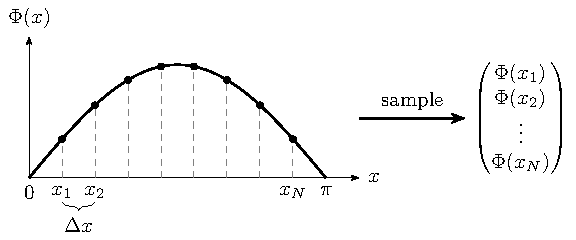
\includegraphics{wavefunction_array.pdf}
    \caption{Wavefunction $\Phi(x) = \sqrt{2/\pi}\,\sin x$ sampled at $N$ points with spacing $\Delta x$. The sampled values form a column vector with $N$ entries. The column vector becomes the continuous function for $\Delta x \to 0$ and $N \to \infty$.}
    \label{fig:array}
\end{figure}

\paragraph{A function is also an abstract vector.} The whole function $\Phi$, rather than a single value $\Phi(x)$, is itself a vector for the same reason as $|\Phi\rangle$. The \textcolor{blue}{square-integrable functions}, with $\int |\Phi(x)|^2\, dx$ finite, form the vector space $L^2$. The sum of two square-integrable functions is square-integrable, a complex multiple of a square-integrable function is square-integrable, and the zero function is the zero vector. The functions, therefore, obey every rule in Table~\ref{tab:axioms}. The inner product in the position basis follows from the completeness relation:
\begin{align*}
    \langle \Psi | \Phi \rangle &= \int dx\, \langle \Psi | x \rangle \langle x | \Phi \rangle \\
    &= \int dx\, \langle x | \Psi \rangle^* \langle x | \Phi \rangle
\end{align*}
\begin{equation}
    \boxed{\langle \Psi | \Phi \rangle = \int dx\, \Psi^*(x)\, \Phi(x)}
\end{equation}
The integral is the continuous version of the sum of products in Section~1, so the integral is the formula of the inner product in the position basis rather than the definition of the inner product. The squared length $\langle \Phi | \Phi \rangle = \int dx\, |\Phi(x)|^2$ is the special case of a state with itself. The map from $|\Phi\rangle$ to $\Phi(x)$ keeps sums, complex multiples and inner products unchanged. The Hilbert space $\mathcal{H}$ and the function space $L^2$ are, therefore, two descriptions of the same vectors. The state vector is the basis-free description, and the wavefunction is the description in the position basis.

\paragraph{The momentum eigenbasis gives another representation of the same state.} The state vector can also be expanded in the \textcolor{blue}{momentum eigenbasis}, in the same way as in the position eigenbasis. \textcolor{red}{The momentum representation is written as $\tilde{\Phi}(p)$, with a tilde, to distinguish it from the position representation $\Phi(x)$.} Each value $\tilde{\Phi}(p)$ is the component of $|\Phi\rangle$ along the momentum eigenstate $|p\rangle$:
\begin{equation}
    \boxed{\tilde{\Phi}(p) = \langle p | \Phi \rangle}
\end{equation}
The position and momentum representations are two lists of components for the same state $|\Phi\rangle$, like the two lists $(v_1, v_2)$ and $(v_1', v_2')$ in Fig.~\ref{fig:bases}.

\paragraph{The position and momentum eigenbases are linked by a unitary transformation.} The position and momentum eigenstates are both orthonormal under the same inner product, with $\langle x | x' \rangle = \delta(x - x')$ and $\langle p | p' \rangle = \delta(p - p')$. The change of basis is a matrix with continuous indices, $U(x, p) = \langle x | p \rangle$. The momentum operator acts as $-i\hbar\, d/dx$ in the position representation, so the eigenvalue equation $\hat p |p\rangle = p |p\rangle$ projected onto $\langle x|$ is a differential equation:
\begin{align*}
    \langle x | \hat p | p \rangle &= -i\hbar \frac{d}{dx} \langle x | p \rangle \\
    &= p\, \langle x | p \rangle
\end{align*}
The solution is a plane wave, $\langle x | p \rangle = C\, e^{ipx/\hbar}$, with a constant $C$. The normalization $\langle p | p' \rangle = \delta(p - p')$ fixes $C$, with the completeness relation of the position eigenbasis and $\int dx\, e^{ikx} = 2\pi\, \delta(k)$:
\begin{align*}
    \langle p | p' \rangle &= \int dx\, \langle p | x \rangle \langle x | p' \rangle \\
    &= |C|^2 \int dx\, e^{i(p' - p)x/\hbar} \\
    &= |C|^2\, 2\pi\hbar\, \delta(p - p')
\end{align*}
The choice of a real, positive $C = 1/\sqrt{2\pi\hbar}$ gives
\begin{equation}
    \boxed{\langle x | p \rangle = \frac{1}{\sqrt{2\pi\hbar}}\, e^{ipx/\hbar}}
\end{equation}
The same calculation is the unitarity condition $U^{\dagger} U = \mathbb{I}$ written with continuous indices. The orthonormality of the momentum eigenbasis is, therefore, not automatic. A momentum formula without the factor $C$ would be off by $2\pi\hbar$ and would describe a different inner product. The momentum representation then follows from the position representation by the completeness relation:
\begin{align*}
    \tilde{\Phi}(p) &= \int dx\, \langle p | x \rangle \langle x | \Phi \rangle \\
    &= \int dx\, \langle x | p \rangle^{*}\, \Phi(x)
\end{align*}
\begin{equation}
    \boxed{\tilde{\Phi}(p) = \frac{1}{\sqrt{2\pi\hbar}} \int dx\, e^{-ipx/\hbar}\, \Phi(x)}
\end{equation}
The change from the position to the momentum representation is, therefore, a \textcolor{blue}{Fourier transform}. The reverse change uses the completeness relation of the momentum eigenbasis, $\int dp\, |p\rangle\langle p| = \mathbb{I}$:
\begin{align*}
    \Phi(x) &= \int dp\, \langle x | p \rangle \langle p | \Phi \rangle \\
    &= \frac{1}{\sqrt{2\pi\hbar}} \int dp\, e^{ipx/\hbar}\, \tilde{\Phi}(p)
\end{align*}
The unitary change of basis keeps the inner product unchanged, so the overlap of two states is the same in both representations:
\begin{align*}
    \langle \Psi | \Phi \rangle &= \int dp\, \langle \Psi | p \rangle \langle p | \Phi \rangle \\
    &= \int dp\, \tilde{\Psi}^{*}(p)\, \tilde{\Phi}(p) \\
    &= \int dx\, \Psi^{*}(x)\, \Phi(x)
\end{align*}
Table~\ref{tab:inner} collects the formulas of the inner product in the position basis, the momentum basis and a discrete orthonormal basis $\{|n\rangle\}$, with the components $c_n = \langle n | \Psi \rangle$ and $d_n = \langle n | \Phi \rangle$. Every momentum eigenstate overlaps every position eigenstate with the same magnitude, $|\langle x | p \rangle| = 1/\sqrt{2\pi\hbar}$. The two bases are, therefore, as far from aligned as possible, and a state that is sharp in one representation is spread over the whole of the other.

\begin{table}[h]
    \centering
    \caption{Formulas of the inner product $\langle \Psi | \Phi \rangle$ in three orthonormal bases.}
    \label{tab:inner}
    \renewcommand{\arraystretch}{1.5}
    \begin{tabular}{lll}
        \toprule
        Basis & Completeness relation & Inner product $\langle \Psi | \Phi \rangle$ \\
        \midrule
        Position $\{|x\rangle\}$ & $\int dx\, |x\rangle\langle x| = \mathbb{I}$ & $\int dx\, \Psi^{*}(x)\, \Phi(x)$ \\
        Momentum $\{|p\rangle\}$ & $\int dp\, |p\rangle\langle p| = \mathbb{I}$ & $\int dp\, \tilde{\Psi}^{*}(p)\, \tilde{\Phi}(p)$ \\
        Discrete $\{|n\rangle\}$ & $\sum_n |n\rangle\langle n| = \mathbb{I}$ & $\sum_n c_n^{*}\, d_n$ \\
        \bottomrule
    \end{tabular}
\end{table}
